
\chapter{Dettagli implementativi del Framework sviluppato}
\label{cap:dettagli}
\lhead{Dettagli implementativi del Framework sviluppato}
In questo capitolo verranno analizzati alcuni dei dettagli implementativi più interessanti.
\rhead{}
\section{Architettura software del tool}
%\rhead{Architettura software del tool}
Nella Figura \ref{fig:arch.soft} viene illustrata una semplificazione dell'architettura software del tool con aggiunta delle interazioni con l'ambiente più interessanti.
\begin{figure}[H]
	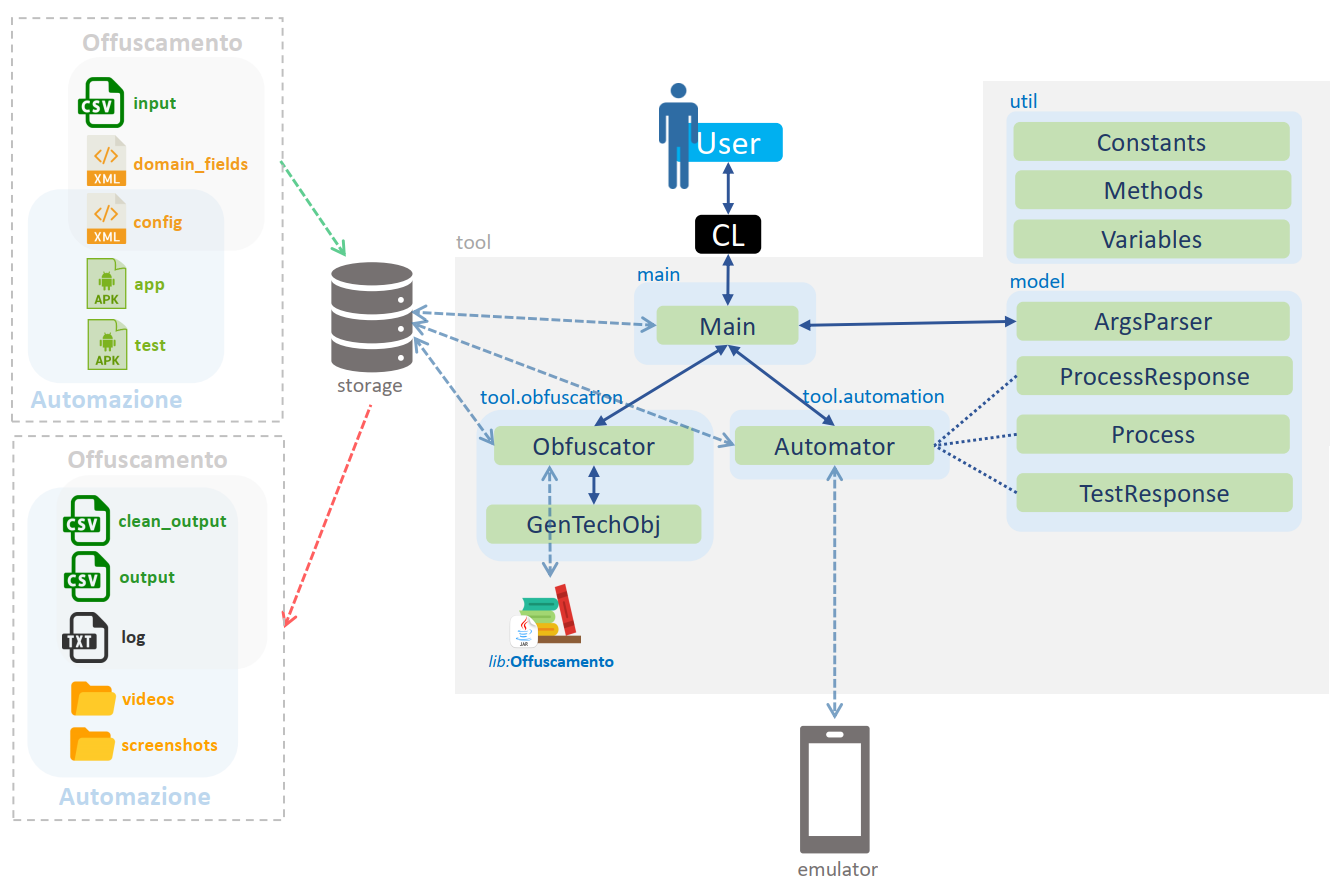
\includegraphics[scale=0.45]{architettura.software}
	\centering
	\caption{Architettura software}
    \label{fig:arch.soft}
\end{figure}

\noindent Come ripetuto più volte, lo strumento deve essere lanciato dall'utente da linea di comando. Il tool interagisce con l'emulatore (su cui esegue i casi di test) e con la memoria (da cui legge e in cui produce file). \\\\ \noindent Brevemente si analizza l'utilità della classi in base al package di appartenenza:


\begin{itemize} [nosep]
\item [$\blacksquare$]  \textbf{\textcolor{gray}{package: }main} \newline
Il package 'main' contiene solamente la classe 'Main'. La classe si interfaccia direttamente con l'utente e svolge la funzione di lettura dei parametri (e lancio del parsing) e chiamata ai metodi in base al comando da eseguire.
\item [$\blacksquare$]  \textbf{\textcolor{gray}{package: }tool.obfuscation} \newline
Il package 'tool.obfuscation' contiene le classi che si occupano di gestire l'intero processo di offuscamento dei dati. Il package si interfaccia con la libreria di offuscamento. 
\item [$\blacksquare$]  \textbf{\textcolor{gray}{package: }tool.automation} \newline
Il package 'tool.automation' contiene solamente la classe 'Automator' che si occupa di gestire l'intero processo di automazione dei test. La classe si interfaccia con l'emulatore gestendo inoltre il suo ciclo di vita.
\item [$\blacksquare$]  \textbf{\textcolor{gray}{package: }util} \newline
Il package 'util' contiene le classi con parametri/metodi utili all'intero tool.
\item [$\blacksquare$]  \textbf{\textcolor{gray}{package: }model} \newline
Il package 'model' contiene le classi che modellano concetti utili ad altre classi.
\end{itemize}

\input capitoli/032-configurazione
\input capitoli/034-lancio

\section{Gestione dell'emulatore per l'automazione dei test}  
%\rhead{Gestione dell'emulatore per l'automazione dei test}
L'automazione dei test è resa possibile dall'utilizzo di un emulatore  e di un gestore dei device che ne permetta un controllo completo.
Per ogni esecuzione della funzionalità di automazione dei test, il tool gestisce il ciclo di vita dell'emulatore seguendo,  in termini genereali, i passi sottostanti:
\begin{enumerate}[nosep]
\item nel caso ci siano emulatori in esecuzione, li chiude;
\item avvia l'emulatore specificato nel file di configurazione;
\item attende che l'emulatore sia stato completamente avviato;
\item porta l'emulatore alla home screen;
\item installa l'APK dell'applicazione (se già installata sull'emulatore, prima la disinstalla);
\item installa l'APK di test dell'applicazione (se già installata sull'emulatore, prima la disinstalla);
\item ottiene la strumentazione dell'APK di test ;
\item per ogni tupla (di parametri) del file di input:
\begin{itemize}[nosep]
\item [1.] elimina i dati dell'applicazione;
\item [2.] lancia il test passando i parametri di esecuzione  (Sezione \ref{pasparam});
\end{itemize}
\end{enumerate}


\section{Passaggio dei parametri alla classe di test}  
%\rhead{Passaggio dei parametri alla classe di test}
\label{pasparam}

Nell'automazione dei test, il tool deve essere in grado di lanciare, per ogni tupla del file di input, un test parametrico. La soluzione adottata prevede di sfruttare la possibilità di passare dei parametri alla strumentazione di test, specificandoli come argomento custom del comando adb che lancia i test sull'emulatore. La classe di test può leggere questi parametri accedendo al bundle degli argomenti della strumentazione (Appendice A - Generazione degli APK - 2.Parametrizzazione della classe di test). I parametri vengono passati nel formato JSON in modo da essere ben organizzati e facilmente leggibili dalla classe di test. 
\\\\
Il comando adb utilizzato per lanciare il test passando i parametri come argomento custom è il seguente:
\begin{itemize}[nosep]
\item []\small{ \textbf{adb shell am instrument -w -r -e clearPackageData true \ul{-e args [parametri]}  -e debug false -e class  testClassName testPackageName/testRunner}}
\end{itemize}
Nel'esecuzione del comando appena illustrato, la stringa \emph{[parametri]} viene sostituita con i parametri in formato JSON compresi tra i singoli apici. Lo strumento, in particolar modo,  crea un oggetto JSON con i parametri da passare e inserisce nel comando la stringa ottenibile dall'oggetto. Un esempio di una stringa valida è: 
\begin{itemize}[nosep]
\item [] '\emph{activityName1="activity1";activityName2="activity2"}'.
\end{itemize} 


\section{Gestione del salvataggio degli screen record}  
%\rhead{Gestione del salvataggio degli screen record}

\label{gsr} 
Per ogni esecuzione della funzionalità di automazione dei test con parametro \emph{screenrecord} impostato a true, il tool :
\begin{enumerate} [nosep]
\item crea la cartella 'videos' nel path interno del device  /sdcard/DCIM (se esiste una cartella con lo stesso nome, prima la elimina);
\item per ogni caso di test:
\begin{itemize} [nosep]
\item [1.]  inizia la registrazione dello schermo prima di lanciare il caso di test;
\item [2.] termina la registrazione dello schermo al termine dell'esecuzione del caso di test;
\item [3.] salva la registrazione dello schermo nella cartella creata al punto 1 (viene utilizzato un identificativo incrementale nel nome - testX.mp4);
\end{itemize}
\item effettua un pull della cartella 'videos' nella cartella di output dell'esecuzione nel package di lancio;
\item elimina la cartella 'videos' dal device.
\end{enumerate}
\bigskip
\noindent Quindi, la registrazione dello schermo inizia prima che l'applicazione venga aperta e si conclude alla sua chiusura . Nel file di output dell'esecuzione \emph{output.csv} viene aggiunta la colonna 'VideoPath' che contiene, per ogni test, il path della relativa registrazione dello schermo. 
\begin{figure}[H]
	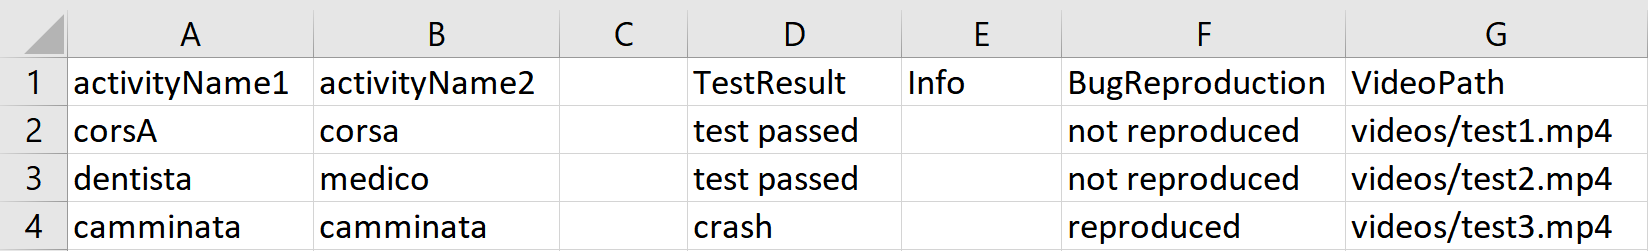
\includegraphics[scale=0.45]{screenrecord.esempio}
	\centering
	\caption{Esempio: \emph{output.csv}}
    \label{fig:resempio}
\end{figure}

\noindent In Figura \ref{fig:resempio} viene illustrato in esempio un file di output per l'esecuzione della funzionalità 'Automatizzazione dei test' con parametro \emph{screenrecord} settato a true.


\section{Gestione del salvataggio degli screenshot}  
%\rhead{Gestione del salvataggio degli screenshot}

\label{gss} 
Il salvataggio di uno screenshot per ogni esecuzione del caso di test, rispetto al salvataggio degli screen record (trattato nella Sezione \ref{gsr}), risulta molto più complicato e richiede un maggiore livello di configurazione. Il tool che gestisce il lancio dei test parametrici non è in grado di conoscere l'esatto momento in cui il bug si presenta (o non si presenta) e non è in grado quindi di effettuare uno screenshot nel momento interessante ai fini dello studio. La soluzione adottata affida la cattura della schermata alla classe di test, in quanto in grado di intervenire in un momento interno all'esecuzione del caso di test. 
\\\\
\noindent\textbf{Comando} \newline
Lo screenshot può essere effettuato attraverso il seguente comando:
\begin{itemize} [nosep]
\item[]  \small{UiDevice device = UiDevice.getInstance(InstrumentationRegistry.getInstrumentation()); \newline
 boolean taked = device.takeScreenshot(new File("/sdcard/DCIM/screenshots/screen.png"));}
\end{itemize}
La cattura dello schermo è resa possibile dall'utilizzo della classe UiDevice offerta da UiAutomator, che è in grado di accedere alle funzionalità e alle informazioni del device su cui viene eseguita la classe di test. Risulta opportuno notare, che l'utilizzo di UiAutomator implica l'utilizzo di AndroidX nel progetto: nel caso così non fosse, è necessario effettuare la migrazione del progetto ad AndroidX (Appendice A - Migrazione del progetto ad AndroidX).\\\\
\bigskip
\noindent\textbf{Struttura della classe di test che effettua lo screenshot}

\begin{figure}[H]
	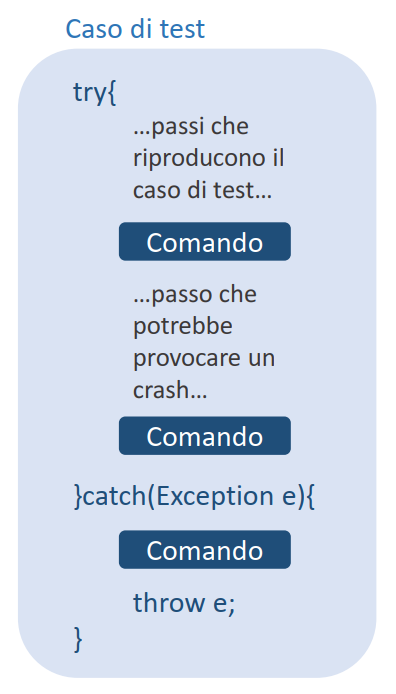
\includegraphics[scale=0.45]{screenshot.classe}
	\centering
	\caption{Struttura della classe che cattura la schermata}
    \label{fig:screens}
\end{figure}

\noindent Il comando appena presentato deve essere posizionato in più punti del metodo che riproduce il caso di test, come esposto in Figura \ref{fig:screens}:
\begin{itemize}
\item [$\blacksquare$] \textbf{nel ramo catch di un blocco try-catch che racchiude tutta il caso di test} \newline
In questo modo, se il caso di test sollevasse un'eccezzione verrebbe effettuato immediatamente uno screenshot. Dopo il comando l'eccezione viene risollevata in modo che sia catturabile dal tool.

\item [$\blacksquare$] \textbf{prima del passo che potrebbe provocare un crash dell'applicazione} \newline
In questo modo, se il caso di test provocasse un crash dell'applicazione senza sollevamento di un'eccezione, sarebbe comunque salvata una schermata del momento antecedente al bug.

\item [$\blacksquare$] \textbf{al termine del caso di test} \newline
In questo modo, anche nel caso in cui il caso di test termini con successo, sarà comunque salvata una schermata del momento antecedente alla chiusura dell'applicazione.
\end{itemize}

\bigskip
\noindent Per ogni esecuzione della funzionalità di automazione dei test con parametro \emph{screenshot} settato a true, il tool :
\begin{enumerate} [nosep]
\item crea la cartella 'screenshots' nel path interno del device  /sdcard/DCIM (se esiste una cartella con lo stesso nome, prima la elimina);
\item al termine dell'esecuzione di ogni caso di test, effettua un pull del file /sdcard/DCIM/
screenshots/screen.png (ultimo screenshot effettuato)  nella cartella di output 'screenshots' nel package di lancio (viene utilizzato un identificativo incrementale nel nome - testX.png);
\item elimina la cartella 'screenshots' dal device.
\end{enumerate}
\bigskip
\noindent Nel file di output dell'esecuzione \emph{output.csv} viene aggiunta la colonna 'ScreenshotPath' che contiene, per ogni test, il path della relativa immagine di cattura dello schermo. 
\begin{figure}[H]
	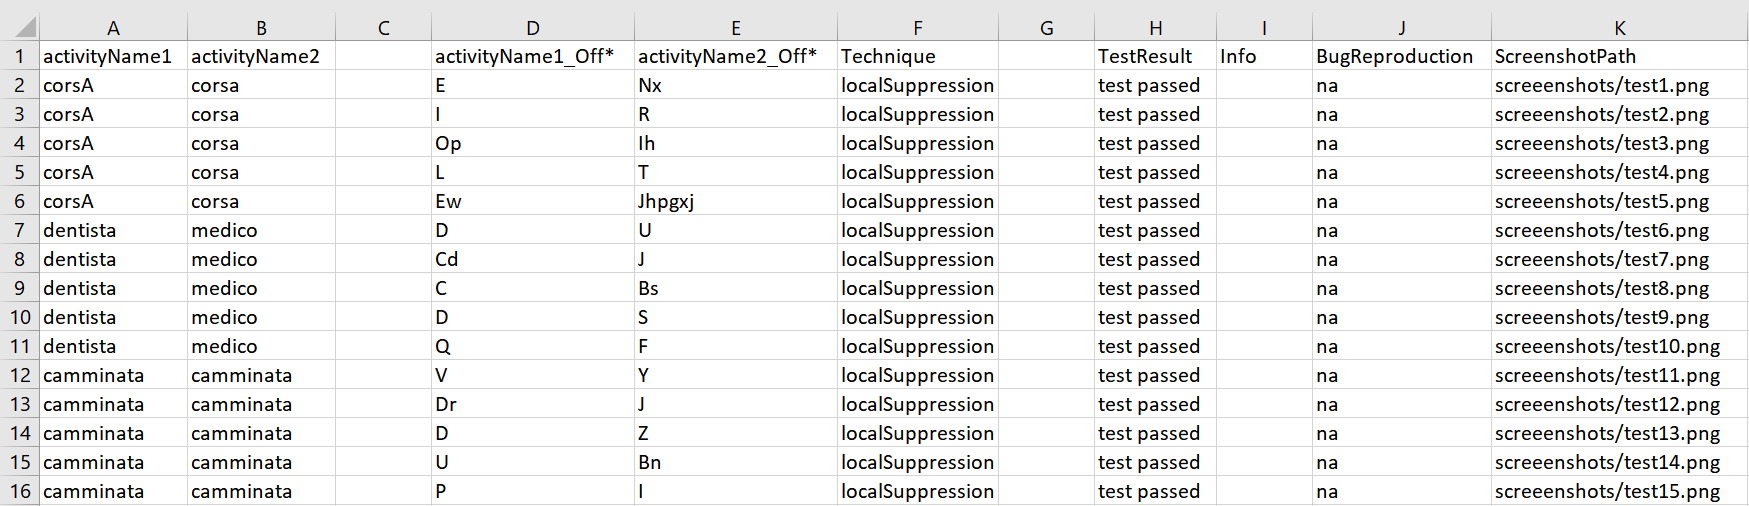
\includegraphics[scale=0.42]{screenshot.esempio}
	\centering
	\caption{Esempio: \emph{output.csv}}
    \label{fig:sesempio}
\end{figure}

\noindent In Figura \ref{fig:sesempio} viene illustrato in esempio un file di output per l'esecuzione della funzionalità 'Offuscamento dei dati e automatizzazione dei test' con parametro \emph{screenshot} settato a true.
